\documentclass{article}
\usepackage[osf]{Baskervaldx} % tosf in text, tlf in math
\usepackage[baskervaldx,bigdelims,vvarbb]{newtxmath} % math italic
                                % letters from Baskervaldx 
\usepackage[cal=boondoxo]{mathalfa} % mathcal from STIX, unslanted a
                                % bit 
\usepackage{inconsolata}
\usepackage{fancyvrb}
\usepackage{xcolor}
\usepackage{tikz}
\usetikzlibrary{positioning,shapes}
\def\Redbf{\color{red}\bfseries}
\def\Red{\color{red}}
\def\Greenbf{\color{green}\bfseries}
\def\Green{\color{green}}
\begin{document}
\title{A tool for redacting the sources:
  \textsl{srcredact}\thanks{This work was commissioned by the US Consumer
  Financial Protection Bureau, United States Treasury}}
\author{Boris Veytsman}
\date{$ $Revision: 1.4 $ $Date: 2015/05/20 23:30:22 $ $}
\maketitle

\clearpage
\tableofcontents

\clearpage

\section{Introduction}
\label{sec:intro}

Many documents containing confidential information exist in several
versions: one for the general public, one for the limited audience (or
even several confidential versions for the different audiences).  In
some cases the desire to have several versions of a document might be
caused not by confidentiality, but by the different needs of
audiences: e.g. an ``executive'' and ``research'' version of the same
white paper.   

One can maintain several versions of the document separately, but this
quickly becomes cumbersome and error-prone.  At some point the
versions drift away too much, and making them close again becomes a
difficult and expensive task.  This is a typical ``anti-pattern'',
well known to programmers.

Therefore the task is to enable the user to have a single source from
which various versions of a document can be produced.

There are different ways to achieve this effect.  The
\emph{output-level} redaction means that we have a specially marked
source file, from which several different PDF files can be produced.  

The \emph{source-level} redaction means that we have one source file,
also specially marked, from which several different \emph{sources} can
be produced.  This means that different co-authors can get different
versions of a source file and work in their own versions of text.
This is the approach taken by the present tool.

One may consider the idea of different co-authors to have different
versions of text to be rather strange.  Why would an author to be
denied the access to a part of her own text?  However, there are
situations where this idea is warranted.  Suppose we have a report
that has classified and non-classified parts.  Suppose also that some
non-classified parts are co-authored by experts that do not have the
privilige to read (all or some) classified parts of the report.  We
want to enable their work on their parts without compromising the
confidentiality of the whole.

\LaTeX\ actually provides some facilities for this approach with its
\verb|\input| and \verb|\include| mechanism.  Indeed, one can put in
the document:
\begin{verbatim}
classified text...

\input{unclassified-part}

classified tex
\end{verbatim}
However, this mechanism allows only limited control over the sources.  

The program \textsl{srcredact} is intended to provide a more
fine-grained control over the included and excluded parts. 

\section{Concept of Operation}
\label{sec:concept}

Let us first discuss a document, that has two versions: classified and
unclassified one.  There are two modes for creation of such document
with the package \textsl{srcredact}.  In the first mode the master
file is a valid \TeX\ file, which provides the full version of the
document, and the redacted version is the file with certain parts
omitted (Figure~\ref{fig:master1st}).  In the second mode some parts
of the redacted version are \emph{not} present in the unredacted
version (Figure~\ref{fig:master2nd}).  These two modes determine two
work flows.  In the first case flow we run \textsl{latex} on the
document to get the full version, \emph{or} \textsl{srcredact} and
then \textsl{latex} to get the redacted (unclassified) version
(Figure~\ref{fig:flow1st}).  In the second case we run
\textsl{srcredact} (with different options) to get either classified
or unclassified versions of the package (Figure~\ref{fig:flow2nd}).  

\begin{figure}
  \centering
  \begin{Verbatim}[commandchars=+^_]
\documentclass{article}

\begin{document}
Common text
+Redbf%<*!unclassified>
+Red^_Classified text
+Redbf%</!unclassified>
\end{document}
  \end{Verbatim}
  \caption{Master document in the first mode}
  \label{fig:master1st}
\end{figure}

\begin{figure}
  \centering
  \begin{Verbatim}[commandchars=+^_]
%<*ALL>
\documentclass{article}

\begin{document}
Common text
%</ALL>
+Redbf%<*classified>
+Red^_Classified version of the text
+Redbf%</!classified>
+Greenbf%<*unclassified>
+Green^_Unclassified version of the text
+Greenbf%</unclassified>
%<*ALL>
\end{document}
%</ALL>
  \end{Verbatim}
  \caption{Master document in the second mode}
  \label{fig:master2nd}
\end{figure}

\begin{figure}
  \centering
  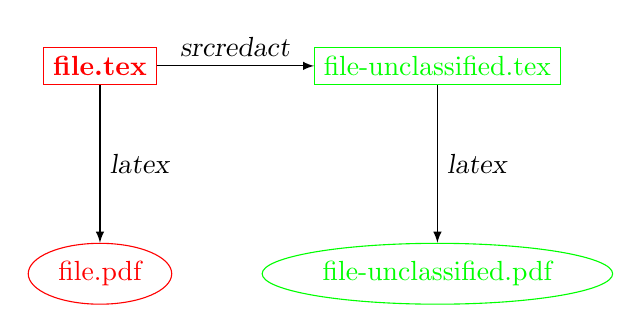
\begin{tikzpicture}
    \node[draw, rectangle, on grid, color=red] (filetex)
    {\color{red}\bfseries file.tex}; 
    \node[draw, ellipse, below=2cm of filetex, on grid,
    color=red] (filepdf) {\color{red}file.pdf};
    \draw[arrows=-latex] (filetex) -- node [right] {\textsl{latex}}
    (filepdf);
    \node[draw,rectangle, right=2 cm of filetex, on grid, color=green]
    (redactedtex)      {\color{green}file-unclassified.tex};
    \draw[arrows=-latex] (filetex) -- node[above] {\textsl{srcredact}}
    (redactedtex); 
    \node[draw, ellipse, below=2 cm of redactedtex, on grid,
    color=green] (redactedpdf) {\color{green}file-unclassified.pdf};  
    \draw[arrows=-latex] (redactedtex) -- node [right] {\textsl{latex}}
    (redactedpdf);
  \end{tikzpicture}
  \caption{Work flow in the first mode.  The red color corresponds to
    the classified material, the green color to the unclassified one.}
  \label{fig:flow1st}
\end{figure}


\begin{figure}
  \centering
  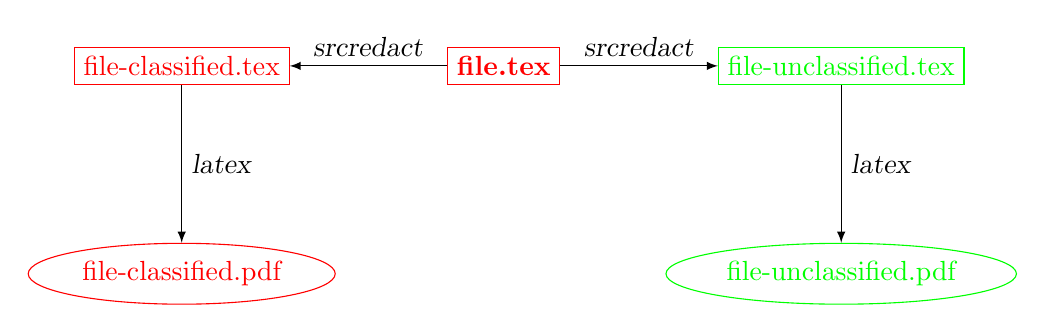
\begin{tikzpicture}
    \node[draw, rectangle, on grid, color=red] (filetex)
    {\color{red}\bfseries file.tex}; 
    \node[draw,rectangle, left=2 cm of filetex, on grid, color=red]
    (secrettex)      {\color{red}file-classified.tex};
    \draw[arrows=-latex] (filetex) -- node[above] {\textsl{srcredact}}
    (secrettex); 
    \node[draw, ellipse, below=2cm of secrettex, on grid,
    color=red] (secretpdf) {\color{red}file-classified.pdf};
    \draw[arrows=-latex] (secrettex) -- node [right] {\textsl{latex}}
    (secretpdf);
    \node[draw,rectangle, right=2 cm of filetex, on grid, color=green]
    (redactedtex)      {\color{green}file-unclassified.tex};
    \draw[arrows=-latex] (filetex) -- node[above] {\textsl{srcredact}}
    (redactedtex); 
    \node[draw, ellipse, below=2 cm of redactedtex, on grid,
    color=green] (redactedpdf) {\color{green}file-unclassified.pdf};  
    \draw[arrows=-latex] (redactedtex) -- node [right] {\textsl{latex}}
    (redactedpdf);
  \end{tikzpicture}
  \caption{Work flow in the second mode.  The red color corresponds to
    the classified material, the green color to the unclassified one.}
  \label{fig:flow2nd}
\end{figure}

In a more complex case we can have more than two versions of the
document, for example, intended for different audiences.  In all cases
we can either plan to a ``full'' version, obtained by \textsl{latex}'ing
the master document, or to assume that no version is the superset of
all other versions, and thus we need \textsl{srcredact} to get any
version of the document.

\section{\textsl{srcredact} man page}
\label{sec:manpage}

The following is the manual page of \textsl{srcredact} tool.

\input{srcredact-man}

%\bibliographystyle{unsrt}
%\bibliography{srcredact}

\end{document}
